\documentclass[conference]{IEEEtran}
\usepackage[T1]{fontenc}
\usepackage{amsmath,amssymb}
\usepackage{booktabs}
\usepackage{multirow}
\usepackage{array}
\usepackage[table]{xcolor}
\usepackage{url}
\usepackage{cite}
\usepackage{tikz}
\usetikzlibrary{positioning,arrows.meta,decorations.pathreplacing,calc,fit}
% Every measured number the paper quotes, in one place. Sources:
%   Jetson: ~/research/measured/<run>/summary.json, pooled over s1-s3
%           (sum tokens / sum time; energy = work-window board DC energy / generated tokens)
%   Pi 5:   ~/Research/measured, pooled over the two subsets with token logs (n=200)
%   gate/diff: benchmark/ae_gate.py
% \pend marks a cell whose run has not finished; nothing in red may be submitted.
\newcommand{\pend}[1]{\textcolor{red}{#1}}

% ---- Jetson Orin Nano 8GB, 15 W, E2B (n=300 each; complete) ----
\newcommand{\EtwoAccL}{52.7}   \newcommand{\EtwoAccG}{53.0}   \newcommand{\EtwoAccA}{53.0}
\newcommand{\EtwoDecL}{23.00}  \newcommand{\EtwoDecG}{25.58}  \newcommand{\EtwoDecA}{29.52}
\newcommand{\EtwoPrmL}{381}    \newcommand{\EtwoPrmG}{1{,}444} \newcommand{\EtwoPrmA}{385}
\newcommand{\EtwoWallL}{31.0}  \newcommand{\EtwoWallG}{28.3}  \newcommand{\EtwoWallA}{24.1}
\newcommand{\EtwoJL}{0.465}    \newcommand{\EtwoJG}{0.446}    \newcommand{\EtwoJA}{0.370}
\newcommand{\EtwoJiL}{0.258}   \newcommand{\EtwoJiG}{0.254}   \newcommand{\EtwoJiA}{0.207}
\newcommand{\EtwoWL}{10.26}    \newcommand{\EtwoWG}{10.86}    \newcommand{\EtwoWA}{10.58}
\newcommand{\EtwoIdent}{300/300}

% ---- Jetson, E4B (complete 2026-10-05) ----
\newcommand{\EfourAccL}{66.0}  \newcommand{\EfourAccG}{65.3}  \newcommand{\EfourAccA}{65.3}
\newcommand{\EfourDecL}{11.62} \newcommand{\EfourDecG}{15.05} \newcommand{\EfourDecA}{17.67}
\newcommand{\EfourPrmL}{381}   \newcommand{\EfourPrmG}{1{,}446} \newcommand{\EfourPrmA}{385}
\newcommand{\EfourWallL}{62.6} \newcommand{\EfourWallG}{51.9} \newcommand{\EfourWallA}{41.6}
\newcommand{\EfourJL}{0.965}   \newcommand{\EfourJG}{0.838}   \newcommand{\EfourJA}{0.676}
\newcommand{\EfourJiL}{0.552}  \newcommand{\EfourJiG}{0.490}  \newcommand{\EfourJiA}{0.396}
\newcommand{\EfourWL}{10.77}   \newcommand{\EfourWG}{11.62}   \newcommand{\EfourWA}{11.39}
\newcommand{\EfourIdent}{300/300}

% ---- headline ratios (S9 vs llama.cpp / vs little-gemma) ----
\newcommand{\EtwoSpL}{1.28}    \newcommand{\EtwoSpG}{1.15}
\newcommand{\EfourSpL}{1.52} \newcommand{\EfourSpG}{1.17}
\newcommand{\EtwoJsav}{20}     \newcommand{\EfourJsav}{30}   % % less J/token than llama.cpp

% ---- Raspberry Pi 5 (llama.cpp, CPU, 3 threads; n=300 accuracy, n=200 rates) ----
\newcommand{\PiEtwoAcc}{51.7}  \newcommand{\PiEtwoDec}{6.87}  \newcommand{\PiEtwoJ}{1.130}  \newcommand{\PiEtwoW}{6.90}
\newcommand{\PiEfourAcc}{65.7} \newcommand{\PiEfourDec}{3.37} \newcommand{\PiEfourJ}{2.223} \newcommand{\PiEfourW}{6.75}

% ---- ablation (mmlupro-ae variants ngram / reuse, s1-s3, n=300; ngram ran 2026-10-05; reuse-only re-run 2026-10-07/08 after the flags bug) ----
% base row = little-gemma (S3): the AE binary with every switch off is byte-identical to it
\newcommand{\AbNgDecEtwo}{29.51} \newcommand{\AbNgPrmEtwo}{1{,}444} \newcommand{\AbNgWallEtwo}{24.8} \newcommand{\AbNgJEtwo}{0.378}
\newcommand{\AbRuDecEtwo}{25.81} \newcommand{\AbRuPrmEtwo}{385} \newcommand{\AbRuWallEtwo}{27.2} \newcommand{\AbRuJEtwo}{0.464$^c$}
\newcommand{\AbNgDecEfour}{17.82} \newcommand{\AbNgPrmEfour}{1{,}444} \newcommand{\AbNgWallEfour}{42.7} \newcommand{\AbNgJEfour}{0.696}
\newcommand{\AbRuDecEfour}{15.47} \newcommand{\AbRuPrmEfour}{385} \newcommand{\AbRuWallEfour}{47.6} \newcommand{\AbRuJEfour}{0.853$^c$}

% ---- where the time goes (pooled n=300, E2B) ----
\newcommand{\PrefShareL}{2.7}   % % of request time in prefill, llama.cpp
\newcommand{\PrefShareG}{3.2}   % little-gemma
\newcommand{\GenTokL}{198{,}706} \newcommand{\GenTokG}{197{,}977}

% ---- iPhone 15 Pro (MLX, GemmaBench; findings/phone, current run per cell; n=300) ----
% decode pooled sum(gt)/sum(gms); energy = whole-phone battery % x capacity estimate / generated tokens
\newcommand{\PhEtwoAcc}{51.0}  \newcommand{\PhEtwoDec}{14.50} \newcommand{\PhEtwoJ}{0.354}
\newcommand{\PhEfourAcc}{66.0} \newcommand{\PhEfourDec}{9.18}  \newcommand{\PhEfourJ}{0.593}

% ---- request-window energy (power integrated over request windows only; J/gen token, pooled s1-s3) ----
\newcommand{\RwEtwoL}{0.458} \newcommand{\RwEtwoG}{0.438} \newcommand{\RwEtwoA}{0.363}
\newcommand{\RwEfourL}{0.948} \newcommand{\RwEfourG}{0.824} \newcommand{\RwEfourA}{0.664}

% ---- llama.cpp + its own n-gram drafting, width 4 (n3m3), n=300, run 2026-10-07/08 ----
\newcommand{\EtwoAccN}{53.3} \newcommand{\EtwoIdN}{29/300$^b$} \newcommand{\EtwoDecN}{26.63} \newcommand{\EtwoPrmN}{381} \newcommand{\EtwoWallN}{27.9} \newcommand{\EtwoWN}{10.84} \newcommand{\EtwoJN}{0.429} \newcommand{\EtwoJiN}{0.228}
\newcommand{\EfourAccN}{65.0} \newcommand{\EfourIdN}{20/300$^b$} \newcommand{\EfourDecN}{13.83} \newcommand{\EfourPrmN}{381} \newcommand{\EfourWallN}{54.3} \newcommand{\EfourWN}{11.53} \newcommand{\EfourJN}{0.871} \newcommand{\EfourJiN}{0.487}

% \needs{...}: work still to do before submission; every one is listed in the
% Open Items section at the end. Nothing in red may be submitted.
\newcommand{\needs}[1]{\textcolor{red}{[#1]}}

\newcommand{\sys}{CoPR}
\newcommand{\ours}{\sys{}\,(ours)}
\definecolor{oursbg}{gray}{0.88}
\newcolumntype{O}{>{\columncolor{oursbg}}c}
\newcommand{\lc}{llama.cpp}
\newcommand{\lgm}{little-gemma}

\begin{document}

\title{Never Compute Twice: Exact-Output Speedups\\for Gemma~4 on Edge Devices}

\author{\IEEEauthorblockN{Rifky Ari Yunanto}
\IEEEauthorblockA{\textit{National Taiwan University of Science and Technology}\\
Taipei, Taiwan\\
rifkyariy@gmail.com}}

\maketitle

\begin{abstract}
An edge agent needs its language model to be fast, and it needs the answers to
stay the same while you make it fast: a cheaper model, a coarser quantization
or a shorter chain of thought all buy speed by changing what the model says. We
show that on a 15\,W edge board, an NVIDIA Jetson Orin Nano 8\,GB, a large share of the available speed can
be bought without changing a single output byte. Two measurements point the
way. First, decode is $\sim$97\,\% of request time, and the fastest Gemma~4
runtime on this board, \lgm{}, wins on decode but re-prefills 3.8$\times$ more
prompt than \lc{}. Second, chain-of-thought replies copy their own context so
much that replaying recorded replies predicts 1.4 tokens per verify pass for a
draft taken straight from that context. \sys{} applies two established
exact techniques to these facts---prompt-lookup drafting, routed through
\lgm{}'s existing batched verify, and shared-prefix KV reuse made exact for
sliding-window ring buffers---without touching a kernel. Over 300 MMLU-Pro
questions per model, \sys{} reproduces \lgm{}'s replies byte for byte (600/600;
\lc{} and \lgm{} themselves agree on only 12\,\%), decodes \EtwoSpL$\times$
(E2B) and \EfourSpL$\times$ (E4B) faster than \lc{}, and spends
\EtwoJsav\,\% and \EfourJsav\,\% less board energy per token. \lc{}'s own
$n$-gram drafting is exact only where it gains 3\,\%; configured for speed it
changes about 90\,\% of replies and still decodes 1.11--1.28$\times$ slower than
\sys{}.
\end{abstract}

\begin{IEEEkeywords}
edge inference, speculative decoding, prompt lookup, KV-cache reuse, energy measurement, edge devices, Jetson Orin Nano
\end{IEEEkeywords}

% ===========================================================================
\section{Introduction}

Agentic systems are moving onto embedded boards---robots, kiosks, offline
assistants---where one general-purpose language model must answer within a
power budget of a few watts. On such hardware, speed is usually traded for
something: a smaller model, more aggressive quantization, a truncated or
disabled reasoning phase. Each of these changes what the model says, and so
each must be re-validated on accuracy, with all the noise that a few hundred
benchmark questions carry.

This paper asks a narrower question: \emph{how much speed is available on an
edge board without changing the output at all?} We answer it on a Jetson Orin
Nano 8\,GB in its 15\,W mode, with Gemma~4~\cite{gemma4} E2B and E4B on
MMLU-Pro~\cite{mmlupro}, comparing the general-purpose runtime \lc{}~\cite{llamacpp}
with \lgm{}~\cite{littlegemma,littlegemmarepo}, a 6,000-line runtime specialized for
the Gemma~4 family.

The answer starts from two measurements on runs we already had
(Sec.~\ref{sec:where}). Decode is about 97\,\% of request time, and \lgm{} is
faster than \lc{} only there; on prefill it is the opposite, because it
re-reads the whole five-shot prompt for every question where \lc{} reuses it.
And the replies themselves are repetitive in a useful way: a chain of thought
restates options, question terms and the fixed phrasing of the few-shot
answers, so much of what the model is about to write is already in its context.

Both observations have a known remedy that leaves greedy output intact.
Speculative decoding~\cite{leviathan2023,chen2023} with greedy verification
accepts a drafted token only where it equals the model's own choice, and
drafting from the context itself---prompt-lookup decoding~\cite{pld},
LLMA~\cite{llma}, SuffixDecoding~\cite{suffixdecoding}---costs nothing to run. Prefix caching~\cite{vllm,sglang}
skips work whose result is already known. The engineering question is whether
they pay on a board with little compute headroom, inside a runtime built around
sliding-window ring buffers. We do not propose a new drafting algorithm; we
contribute:

\begin{itemize}
\item \textbf{\sys{}}: an implementation of prompt-lookup drafting through
\lgm{}'s existing batched verify kernel, and a shared-prefix KV snapshot that is
exact for sliding-window rings---host-side code only (Sec.~\ref{sec:design}).
\item \textbf{Byte identity as the quality standard.} Every reply is compared
with the baseline runtime's reply to the same question. Two engines on the same
weights agree on only 12\,\% of replies, so a 600/600 match is strong evidence
that nothing but speed changed (Sec.~\ref{sec:method}).
\item \textbf{A measured comparison and ablation} of three engines---and of
\lc{}'s own $n$-gram drafting---on identical
weights, prompts, subsets and clock caps, with accuracy, decode rate, prompt
tokens processed and board energy per token from the same run
(Sec.~\ref{sec:results}).
\item \textbf{Two practical findings}: the best verify width is a property of
the board's kernels (3 on this GPU, a predicted 4 on a Raspberry~Pi~5 CPU),
and gains can be predicted from logged replies before any device time is spent.
\end{itemize}

% ===========================================================================
\section{Background}

\textbf{Speculative decoding.} A drafter proposes $k$ tokens; the target model
scores all of them in one pass and keeps the longest prefix it agrees
with~\cite{leviathan2023,chen2023}. Drafters range from small models to extra
heads (Medusa~\cite{medusa}, EAGLE~\cite{eagle}) and model-free schemes such as
lookahead decoding~\cite{lookahead} and prompt-lookup decoding~\cite{pld}, which
copies the continuation of an earlier $n$-gram match; LLMA~\cite{llma} copies
spans from reference documents and SuffixDecoding~\cite{suffixdecoding} matches
against suffix trees of earlier outputs. \lc{} itself ships several $n$-gram
drafting modes (\texttt{--spec-type ngram-*}). With greedy verification
the output is exactly the greedy output; only the number of target passes per
token changes.

\textbf{Prefix caching.} Serving systems reuse the KV state of shared prompt
prefixes (vLLM~\cite{vllm}, SGLang~\cite{sglang}); \lc{}'s server keeps the
previous request's cache and reuses its longest common prefix. Gemma's
sliding-window layers complicate this: a runtime that stores them as ring
buffers overwrites prefix rows as a reply grows.

\textbf{\lgm{}.} \lgm{} trades generality for one model family: a CUDA graph
captured once per token, fused Gemma-specific kernels, aligned K-quant weight
loads, on-device greedy selection and ring-buffered sliding-window
caches~\cite{littlegemmarepo}. Its authors target voice latency. It ships a
batched verify kernel for Gemma's multi-token-prediction (MTP) head, which is
what makes a model-free drafter cheap to add.

% ===========================================================================
\section{Where the Time Goes}\label{sec:where}

\begin{table}[t]
\caption{Baseline anatomy, Gemma~4 E2B on the Jetson Orin Nano at 15\,W, 300 MMLU-Pro questions}
\label{tab:where}
\centering\footnotesize
\begin{tabular}{@{}lcc@{}}
\toprule
& \lc{} & \lgm{} \\
\midrule
Generated tokens & \GenTokL & \GenTokG \\
Decode rate (tok/s) & \EtwoDecL & \EtwoDecG \\
Prompt tokens prefilled / question & \EtwoPrmL & \EtwoPrmG \\
Share of request time in prefill (\%) & \PrefShareL & \PrefShareG \\
Accuracy (\%) & \EtwoAccL & \EtwoAccG \\
\bottomrule
\end{tabular}
\end{table}

Table~\ref{tab:where} decomposes the two baselines on E2B. Both generate almost
the same number of tokens, and both spend about 97\,\% of request time
generating them, so decode rate decides wall time. \lgm{} decodes 11\,\% faster
(30\,\% on E4B) and is correspondingly faster per question, but it prefills
3.8$\times$ more prompt: it starts every question from an empty cache, while
\lc{} reuses the five-shot prefix the previous question left behind. Prefill
is cheap on this GPU, so this costs only a few percent---yet it is the one
column on which the faster engine loses.

The second observation concerns what is generated. Because greedy output is
deterministic, the effect of any drafter can be computed exactly from recorded
replies: a draft would have been accepted exactly where it equals the recorded
next tokens. Replaying \lgm{}'s 300 recorded E2B replies with a 3-gram lookup
over prompt and reply gives 1.29, 1.41, 1.48 and 1.52 tokens per verify pass at
block widths 2--5, with a match on about 45\,\% of steps. The 17 replies that
run into the 2{,}048-token cap barely move this (1.39 at width~3 without them),
so the effect is not an artefact of degenerate loops. The same replay shows
that stopping at the first ``answer is (X)''---exact for the score---would save
only 1.0\,\% of tokens, which is why we did not pursue it.

% ===========================================================================
\section{Design}\label{sec:design}

\sys{} is \lgm{} at a pinned commit plus one patch to its socket server and
prefix-save routine. Kernels, sampling and tokenizer are untouched; both
mechanisms are switches, off by default.

\begin{figure}[t]
\centering
\resizebox{\columnwidth}{!}{%
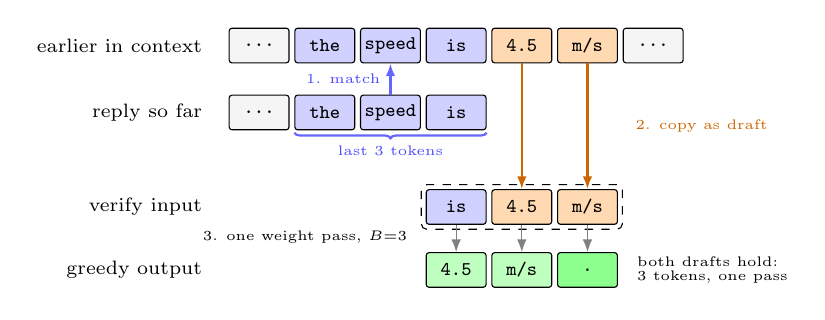
\begin{tikzpicture}[
  tok/.style={draw,rounded corners=1pt,minimum height=4.4mm,minimum width=7.6mm,inner sep=1pt,font=\scriptsize\ttfamily},
  ctx/.style={tok,fill=gray!8},
  key/.style={tok,fill=blue!18},
  cp/.style={tok,fill=orange!30},
  ok/.style={tok,fill=green!25},
  new/.style={tok,fill=green!45},
  lab/.style={font=\scriptsize,anchor=east},
  >={Latex[length=1.6mm]}, node distance=0.6mm]
% row 1: earlier in the context
\node[lab] at (-0.15,0) {earlier in context};
\node[ctx] (a0) at (0.45,0) {...};
\node[key,right=of a0] (a1) {the};
\node[key,right=of a1] (a2) {speed};
\node[key,right=of a2] (a3) {is};
\node[cp,right=of a3]  (a4) {4.5};
\node[cp,right=of a4]  (a5) {m/s};
\node[ctx,right=of a5] (a6) {...};
% row 2: reply so far (its last 3 tokens sit under their earlier match)
\node[lab] at (-0.15,-0.85) {reply so far};
\node[ctx] (b0) at (0.45,-0.85) {...};
\node[key,right=of b0] (b1) {the};
\node[key,right=of b1] (b2) {speed};
\node[key,right=of b2] (b3) {is};
\draw[decorate,decoration={brace,mirror,amplitude=2pt},thick,blue!60]
  ($(b1.south west)+(0,-0.03)$) -- ($(b3.south east)+(0,-0.03)$)
  node[midway,below=1pt,font=\tiny,blue!70] {last 3 tokens};
\draw[->,blue!60,thick] (b2.north) -- node[left,font=\tiny,blue!70]{1. match} (a2.south);
% row 3: verify (drafts directly under their source)
\node[lab] at (-0.15,-2.05) {verify input};
\node[key] (v0) at (a3 |- 0,-2.05) {is};
\node[cp]  (v1) at (a4 |- 0,-2.05) {4.5};
\node[cp]  (v2) at (a5 |- 0,-2.05) {m/s};
\draw[->,orange!80!black,thick] (a4.south) -- (v1.north);
\draw[->,orange!80!black,thick] (a5.south) -- (v2.north);
\node[font=\tiny,orange!80!black,anchor=west] at ($(a5.south east)!0.5!(v2.north east)+(0.1,0)$) {2. copy as draft};
\node[draw,dashed,rounded corners=2pt,fit=(v0)(v2),inner sep=1.6pt] (vb) {};
\node[font=\tiny,anchor=east] at ($(vb.west)+(-0.05,-0.38)$) {3. one weight pass, $B{=}3$};
% row 4: greedy outputs
\node[lab] at (-0.15,-2.85) {greedy output};
\node[ok]  (o0) at (v0 |- 0,-2.85) {4.5};
\node[ok]  (o1) at (v1 |- 0,-2.85) {m/s};
\node[new] (o2) at (v2 |- 0,-2.85) {.};
\foreach \i in {0,1,2} \draw[->,gray] (v\i.south) -- (o\i.north);
\node[font=\tiny,anchor=west,align=left] at ($(o2.east)+(0.12,0)$)
  {both drafts hold:\\[-1pt]3 tokens, one pass};
\end{tikzpicture}}
\caption{Prompt-lookup drafting with greedy verification. (1) The last three
tokens of the reply are matched against their most recent earlier occurrence in
prompt or reply. (2) The tokens that followed it become the draft. (3) One
batched forward pass computes the model's own greedy choice after every input
position. Drafts are accepted left to right while they equal those choices; the
first mismatch is replaced by the model's choice and the rest discarded, so the
emitted text is exactly what one-token-at-a-time greedy decoding produces. Here
both drafts hold and the pass also yields the next token.}
\label{fig:lookup}
\end{figure}

\subsection{Prompt-lookup drafting}
Figure~\ref{fig:lookup} shows one step. At each decode step the engine holds the token history (prompt and reply so
far). It searches backwards for the most recent earlier occurrence of the last
three tokens, falling back to two, and proposes the up to $B{-}1$ tokens that
followed it. The proposal, padded to the verify width $B$, goes through the
existing batched verify, which computes the greedy successor of every position
in one weight pass and accepts the longest matching prefix. A step without a
match decodes normally; a failed lookup costs one scan of at most 8{,}192
tokens, negligible next to a 40\,ms forward pass.

\begin{figure}[t]
\centering
\resizebox{\columnwidth}{!}{%
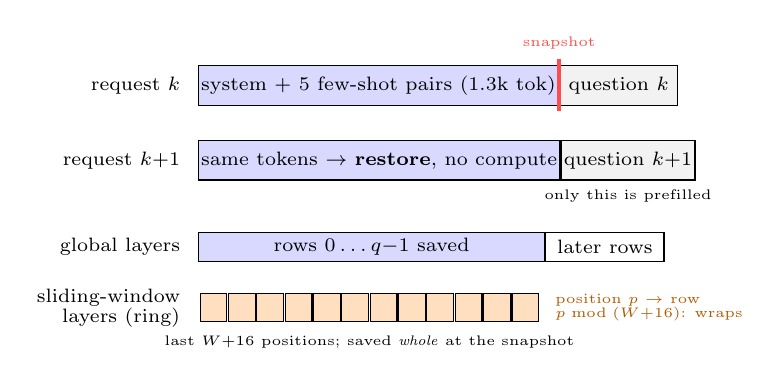
\begin{tikzpicture}[
  seg/.style={draw,minimum height=5mm,inner sep=1pt,font=\scriptsize},
  lab/.style={font=\scriptsize,anchor=east},
  >={Latex[length=1.6mm]}]
% request k
\node[lab] at (-0.1,0) {request $k$};
\node[seg,fill=blue!15,minimum width=4.4cm,anchor=west] (pk) at (0,0) {system + 5 few-shot pairs (1.3k tok)};
\node[seg,fill=gray!10,minimum width=1.5cm,anchor=west] (qk) at (pk.east) {question $k$};
\draw[very thick,red!70] (pk.north east) ++(0,0.08) -- ++(0,-0.66);
\node[font=\tiny,red!70,anchor=south] at ($(pk.north east)+(0,0.08)$) {snapshot};
% request k+1
\node[lab] at (-0.1,-0.95) {request $k{+}1$};
\node[seg,fill=blue!15,minimum width=4.4cm,anchor=west] (pk1) at (0,-0.95) {same tokens $\to$ \textbf{restore}, no compute};
\node[seg,fill=gray!10,minimum width=1.5cm,anchor=west] (qk1) at (pk1.east) {question $k{+}1$};
\node[font=\tiny,anchor=north] at (qk1.south) {only this is prefilled};
% KV layout
\node[lab] at (-0.1,-2.05) {global layers};
\node[seg,fill=blue!15,minimum width=4.4cm,anchor=west,minimum height=3.6mm] (g) at (0,-2.05) {rows $0\ldots q{-}1$ saved};
\node[seg,fill=white,minimum width=1.5cm,anchor=west,minimum height=3.6mm] at (g.east) {later rows};
\node[lab] at (-0.1,-2.7) {sliding-window};
\node[lab] at (-0.1,-2.95) {layers (ring)};
\foreach \i in {0,...,11} {
  \node[draw,minimum width=3.4mm,minimum height=3.6mm,inner sep=0pt,fill=orange!25] (r\i) at (0.2+\i*0.36,-2.82) {};
}
\node[font=\tiny,anchor=west,align=left,orange!70!black] at ($(r11.east)+(0.08,0)$) {position $p$ $\to$ row\\[-1pt]$p \bmod (W{+}16)$: wraps};
\node[font=\tiny,anchor=north,align=center] at ($(r5.south)+(0.18,-0.05)$) {last $W{+}16$ positions; saved \emph{whole} at the snapshot};
\end{tikzpicture}}
\caption{Shared-prefix KV reuse. A request that misses the cached prefix saves
the KV state at the start of its final user turn; the next request whose
prompt begins with exactly those tokens restores it and prefills only its
question. Global-attention rows below the snapshot are never overwritten by
later positions of the same subject, but the sliding-window layers are rings
that a long reply wraps over, so the ring is stored whole---its exact content
at the snapshot position---and rewritten on restore.}
\label{fig:reuse}
\end{figure}

\subsection{Shared-prefix KV reuse}
Figure~\ref{fig:reuse} shows the mechanism. Prompts for one MMLU-Pro subject share a system turn and five few-shot pairs
(1--2k tokens) and differ only in the final user turn. When a request does not
start with the cached prefix, \sys{} prefills up to the start of its final user
turn, saves the KV state there, and continues; the next request that begins
with exactly those tokens restores it and prefills only its own question.
Global-attention layers keep every row, but sliding-window layers are rings that
wrap during a long reply, so the snapshot stores each ring whole---its exact
content at the snapshot position---and restore rewrites it. Buffers are
allocated once (39\,MiB on E2B).

\subsection{Why the output cannot change, and how we check}
A draft token is kept only where it equals the verify pass's own greedy choice,
and a restored prefix holds the very rows a fresh prefill writes. We do not
rely on the argument: every \sys{} reply is compared byte for byte with
\lgm{}'s reply to the same question (Sec.~\ref{sec:method}).

\subsection{What we deliberately left out}
Gemma's MTP draft head could feed the same verify, but no run in this paper
uses it---neither baseline nor \sys{}---so that every gain reported comes from
the two mechanisms above and not from a stock feature the baselines left off.

% ===========================================================================
\section{Methodology}\label{sec:method}

\begin{table}[t]
\caption{Benchmark protocol, identical for every engine}
\label{tab:protocol}
\centering\footnotesize
\begin{tabular}{@{}ll@{}}
\toprule
Task & MMLU-Pro, 5-shot CoT, lm-eval~\cite{lmeval} \texttt{mmlu\_pro} \\
Questions & 3 disjoint stratified subsets of 100 (seeded); $n{=}300$ \\
Models & Gemma~4 E2B, E4B; same QAT \texttt{UD-Q4\_K\_XL} GGUF \\
Decoding & greedy; 2{,}048-token answer cap; 8{,}192 context \\
Thinking & off (\texttt{-rea off}; no \texttt{<|think|>} turn) \\
Device & Jetson Orin Nano 8\,GB, 15\,W mode \\
Clock caps & GPU 612\,MHz, CPU 1{,}497.6\,MHz (checked per run) \\
Scoring & exact match on the first \texttt{answer is (X)} \\
\bottomrule
\end{tabular}
\end{table}

\textbf{Engines.} \emph{\lc{}} (CUDA, all layers on GPU, host prompt cache
disabled); \emph{\lgm{}} (stock, behind an OpenAI-compatible shim whose chat
rendering is tested byte-identical to \lc{}'s template); \emph{\sys{}} (\lgm{}
+ \texttt{-reuse -ngram -block 3}). All load the same GGUF file. Each run's
serving command line is captured while it is live and diffed against a declared
configuration before the run counts.

\textbf{Quality.} Accuracy carries sampling uncertainty of about $\pm$5.6
points at $n{=}300$; paired engine comparisons use McNemar's test. For \sys{}
the standard is stricter: every reply must equal \lgm{}'s byte for byte. This
is a meaningful test only because different engines on the same weights rarely
agree---\lc{} and \lgm{} produce identical replies on 12 of 100 questions---so
an engine that changed anything would show it.

\textbf{Energy and speed.} A 1\,Hz sampler reads board power from the INA3221
\texttt{VDD\_IN} rail (board DC input, excluding power-supply loss; not wall
power) together with GPU and CPU utilization and frequency, temperatures,
throttle flags and memory. Energy is the trapezoidal integral over the
command's working window, excluding 30\,s idle baselines recorded before and
after. We report energy per generated token, total and above idle. Rates are
pooled ratios ($\sum$tokens$/\sum$time) of each engine's own per-request
timings; prompt tokens \emph{processed} count only tokens actually prefilled.
Repeating a full \sys{} run three days later (E2B, s1) reproduced all 100
replies byte for byte and decode within 0.8\,\% (29.78 vs.\ 29.54\,tok/s); wall
time differed by 3\,\%, and energy per token by 9\,\% (6\,\% above idle),
tracking a higher idle floor (5.01 vs.\ 4.55\,W) and a warmer board (62 vs.\
60\,$^\circ$C) that day. Speed comparisons across days are therefore tight;
energy comparisons across days carry a band of about $\pm$9\,\%, which is why
Table~\ref{tab:lcngram} compares energy within one day. The working window
includes model load and the gaps between requests; integrating power over the
request windows alone changes energy per token by only 1--2\,\% for every
engine (\sys{} \RwEtwoA{} vs.\ \lc{} \RwEtwoL\,J on E2B, \RwEfourA{} vs.\
\RwEfourL\,J on E4B), so the comparison does not depend on that choice.

\textbf{Clock state, and a near miss.} After one reboot the board's
power-mode service failed silently: the mode query still reported 15\,W, but
the GPU ran at 1{,}020\,MHz under a \emph{performance} governor, and plain
decode came out $\sim$1.6$\times$ faster than in every earlier run. Had we not
compared against the baselines' telemetry, that factor would have been credited
to the engine. All results here are at the 15\,W caps, confirmed against the
baselines' recorded GPU clock (612\,MHz under load); the run queue now refuses
to start whenever the kernel-enforced caps differ from those the active power
mode declares.

% ===========================================================================
\section{Results}\label{sec:results}

\begin{table*}[t]
\caption{Engines on the Jetson Orin Nano 8\,GB at 15\,W, MMLU-Pro, $n{=}300$ per cell.
Energy is board DC energy over the working window per generated token. \textbf{Bold}: best in row, whichever engine; shaded: the
proposed system. The \lc{} column runs without speculative decoding;
\lc{}+$n$-gram is \lc{}'s own drafting at its fastest setting (width~4, not
exact; run Oct~7--8, see Table~\ref{tab:lcngram} for the other settings).}
\label{tab:main}
\centering
\setlength{\tabcolsep}{3.8pt}
\begin{tabular}{@{}l cccO cccO@{}}
\toprule
& \multicolumn{4}{c}{Gemma~4 E2B} & \multicolumn{4}{c}{Gemma~4 E4B} \\
\cmidrule(lr){2-5}\cmidrule(lr){6-9}
& \lc{} & \lc{}+$n$-gram & \lgm{} & \ours & \lc{} & \lc{}+$n$-gram & \lgm{} & \ours \\
\midrule
Accuracy (\%)$^g$              & \EtwoAccL & \EtwoAccN & \EtwoAccG & \EtwoAccA & \EfourAccL & \EfourAccN & \EfourAccG & \EfourAccA \\
Replies identical to \lgm{}    & 12/100$^a$ & \EtwoIdN & -- & \textbf{\EtwoIdent} & -- & \EfourIdN & -- & \textbf{\EfourIdent} \\
Decode (tok/s)                 & \EtwoDecL & \EtwoDecN & \EtwoDecG & \textbf{\EtwoDecA} & \EfourDecL & \EfourDecN & \EfourDecG & \textbf{\EfourDecA} \\
Prompt tokens processed / q    & \textbf{\EtwoPrmL} & \textbf{\EtwoPrmN} & \EtwoPrmG & \EtwoPrmA & \textbf{\EfourPrmL} & \textbf{\EfourPrmN} & \EfourPrmG & \EfourPrmA \\
Wall time / question (s)       & \EtwoWallL & \EtwoWallN & \EtwoWallG & \textbf{\EtwoWallA} & \EfourWallL & \EfourWallN & \EfourWallG$^b$ & \textbf{\EfourWallA} \\
Mean power, generating (W)     & \textbf{\EtwoWL} & \EtwoWN & \EtwoWG & \EtwoWA & \textbf{\EfourWL} & \EfourWN & \EfourWG & \EfourWA \\
Energy / gen.\ token (J)       & \EtwoJL & \EtwoJN & \EtwoJG & \textbf{\EtwoJA} & \EfourJL & \EfourJN & \EfourJG & \textbf{\EfourJA} \\
\quad above idle (J)           & \EtwoJiL & \EtwoJiN & \EtwoJiG & \textbf{\EtwoJiA} & \EfourJiL & \EfourJiN & \EfourJiG & \textbf{\EfourJiA} \\
\bottomrule
\multicolumn{9}{@{}l}{\footnotesize $^a$ E2B, subset s1, compared with the same tool.
$^b$ One subset re-sent 5 prompts (105 requests); per-question figures divide by its 100 questions.}\\
\multicolumn{9}{@{}l}{\footnotesize $^f$ Identical to \lc{} without drafting, not to \lgm{}.
$^g$ Not bolded: all engines are statistically tied (Sec.~\ref{sec:results}).}
\end{tabular}
\end{table*}

\subsection{Quality first: nothing changed}
On both models, \sys{} answers all 300 questions with exactly \lgm{}'s replies
(Table~\ref{tab:main}), and so do the 600 ablation runs: 1{,}200 replies in all,
none different. On E2B its total generated-token count is identical too
(197{,}977), as byte identity requires. Its accuracy is therefore \lgm{}'s:
53.0\,\% on E2B, statistically tied with \lc{}'s 52.7\,\% (paired over the
same questions, 14 right only under \lgm{} and 13 only under \lc{}; exact
McNemar $p{=}1.00$), and 65.3\,\% on E4B against \lc{}'s 66.0\,\%.

\subsection{Speed and energy}
With the output fixed, \sys{} decodes \EtwoSpL$\times$ faster than \lc{} and
\EtwoSpG$\times$ faster than \lgm{} on E2B (\EfourSpL$\times$ and
\EfourSpG$\times$ on E4B). Reuse brings prompt tokens processed from \lgm{}'s
\EtwoPrmG{} per question down to \EtwoPrmA{}, level with \lc{}, removing the
one cost on which \lgm{} trailed. Wall time per question falls 22\,\% against
\lc{} and 15\,\% against \lgm{} on E2B, and 34\,\% and 20\,\% on E4B. Board
power while generating barely moves (10.3--11.6\,W), so energy follows time:
per generated token, \sys{} uses \EtwoJsav\,\% (E2B) and \EfourJsav\,\% (E4B)
less than \lc{}, and 17\,\% and 19\,\% less than \lgm{}. The gain is larger on
E4B against \lc{} because \lgm{}'s own decode advantage is larger there.

\subsection{Against \lc{}'s own $n$-gram drafting}

\begin{table}[t]
\caption{\lc{}'s own $n$-gram drafting (\texttt{--spec-type ngram-simple})
against \sys{}, E2B, subset s1 ($n{=}100$). ``Exact'': replies identical to the
same engine without drafting. Rows of the same date share the board's idle floor.
Bold: best per column; accuracy not bolded (all tied).}
\label{tab:lcngram}
\centering\footnotesize
\setlength{\tabcolsep}{2.6pt}
\begin{tabular}{@{}lcccccc@{}}
\toprule
& Exact & Acc. & Decode & Wall & J/tok & above \\
& & (\%) & tok/s & s/q & & idle \\
\midrule
\lc{}, no drafting$^\ddagger$ & --      & 56 & 23.04 & 27.9 & 0.466 & 0.259 \\
\lc{} $n$-gram, width 3 & \textbf{100/100} & 56 & 23.80 & 27.4 & 0.491 & 0.266 \\
\lc{} $n$-gram, width 4 & 8/100   & 56 & 26.97 & 26.1 & 0.424 & 0.225 \\
\lc{} $n$-gram, stock & 9/100   & 53 & 25.15 & 26.8 & 0.458 & 0.249 \\
\rowcolor{oursbg}\ours, width 3$^\ddagger$ & \textbf{100/100} & 54 & 29.54 & \textbf{23.8} & \textbf{0.370} & \textbf{0.207} \\
\rowcolor{oursbg}\ours, repeat & \textbf{100/100} & 54 & \textbf{29.78} & 24.6 & 0.404 & 0.219 \\
\bottomrule
\multicolumn{7}{@{}l}{\footnotesize $^\ddagger$ Run Sep~22 and Oct~4; all other rows Oct~7.}\\
\end{tabular}
\end{table}

\lc{} ships its own $n$-gram drafting, so the fair question is whether \sys{}
beats \lc{} \emph{with} it. Table~\ref{tab:lcngram} runs it on subset s1 in
three configurations: matched to \sys{} (3-token lookup, width~3), one width
wider, and with \lc{}'s stock settings (12-token lookup, up to 48-token
drafts). At width~3 it is exact---all 100 replies equal \lc{}'s without
drafting---but gains only 3\,\% in decode and costs slightly more energy per
token. At width~4 and with stock settings it is faster (+17\,\% and +9\,\%), but
no longer exact: only 8 and 9 of 100 replies match plain \lc{}, consistent with
its CUDA path computing a 4-token batch with a different kernel than a single
token. Accuracy is unaffected (56 vs.\ 56; four questions flip each way, exact
McNemar $p{=}1.00$), so the change is a numerical one, not a quality loss---but
it is a loss of exactness. Against the fastest of these, run on the same day,
\sys{} decodes 10\,\% faster (29.78 vs.\ 26.97\,tok/s), finishes questions 6\,\%
sooner and uses 5\,\% less energy per token (2\,\% above idle), while its
replies stay byte-identical. Over all 300 questions (Table~\ref{tab:main}) the
picture holds on both models: \lc{} at width~4 changes 271 of 300 E2B replies
and 280 of 300 E4B replies relative to its own plain decoding, with accuracy
tied (53.3 vs.\ 52.7\,\% and 65.0 vs.\ 66.0\,\%; McNemar $p{=}0.86$ and
$0.69$), and decodes 16\,\% and 19\,\% faster than without drafting. \sys{}
still decodes 1.11$\times$ and 1.28$\times$ faster than it, and answers
questions 14\,\% and 23\,\% sooner.

\subsection{Ablation}

\begin{table}[t]
\caption{Ablation, $n{=}300$ per row. The first row is \lgm{} (S3); \sys{} with
every switch off reproduces it byte for byte. Every row's replies are
byte-identical to \lgm{}'s (1{,}800 replies). Bold: best per column within a model.}
\label{tab:ablation}
\centering\footnotesize
\setlength{\tabcolsep}{3pt}
\begin{tabular}{@{}l cccc@{}}
\toprule
& Decode & Prompt & Wall & J / \\
& (tok/s) & tok / q & s / q & tok \\
\midrule
\multicolumn{5}{@{}l}{\emph{Gemma~4 E2B}} \\
\lgm{} (no switches)   & \EtwoDecG & \EtwoPrmG & \EtwoWallG & \EtwoJG \\
+ prompt lookup        & \AbNgDecEtwo & \AbNgPrmEtwo & \AbNgWallEtwo & \AbNgJEtwo \\
+ prefix reuse         & \AbRuDecEtwo & \textbf{\AbRuPrmEtwo} & \AbRuWallEtwo & \AbRuJEtwo \\
\rowcolor{oursbg}+ both (\ours)        & \textbf{\EtwoDecA} & \textbf{\EtwoPrmA} & \textbf{\EtwoWallA} & \textbf{\EtwoJA} \\
\midrule
\multicolumn{5}{@{}l}{\emph{Gemma~4 E4B}} \\
\lgm{} (no switches)   & \EfourDecG & \EfourPrmG & \EfourWallG & \EfourJG \\
+ prompt lookup        & \textbf{\AbNgDecEfour} & \AbNgPrmEfour & \AbNgWallEfour & \AbNgJEfour \\
+ prefix reuse         & \AbRuDecEfour & \textbf{\AbRuPrmEfour} & \AbRuWallEfour & \AbRuJEfour \\
\rowcolor{oursbg}+ both (\ours)        & \EfourDecA & \textbf{\EfourPrmA} & \textbf{\EfourWallA} & \textbf{\EfourJA} \\
\bottomrule
\multicolumn{5}{@{}l}{\footnotesize $^c$ Run Oct~7--8 at a higher idle floor; within the}\\
\multicolumn{5}{@{}l}{\footnotesize \phantom{$^c$} $\pm$9\,\% cross-day energy band (Sec.~\ref{sec:method}).}
\end{tabular}
\end{table}

Table~\ref{tab:ablation} separates the two mechanisms. Prompt lookup alone
delivers nearly all of the decode gain---29.51 against 29.52\,tok/s on E2B,
17.82 against 17.67 on E4B, equal within run-to-run variation---and most of
the wall-clock and energy gain: $-$12\,\% and $-$18\,\% wall time per
question, $-$15\,\% and $-$17\,\% energy per token against \lgm{}. Reuse acts
on prefill only: comparing the full system with lookup alone, it cuts prompt
tokens processed by 73\,\% and adds a further 3\,\% on wall time and 2--3\,\%
on energy per token. The two compose as their phases suggest, almost additively.
Reuse alone leaves decode unchanged (25.81 and 15.47\,tok/s against \lgm{}'s
\EtwoDecG{} and \EfourDecG{}), cuts prompt tokens processed by 73\,\%, and
shortens each question by 4\,\% on E2B and 8\,\% on E4B, where prefill is
slower; it is the full system minus lookup, as expected. Its own energy effect
is smaller than the $\pm$9\,\% band between days on which the rows were run, so
the table cannot resolve it. (These six runs first failed at start-up: the run
script passed the single flag \texttt{-reuse} as a separate argument, which the
shim's argument parser read as an option. They are archived and were re-run
after the fix.)

\subsection{Choosing the verify width}\label{sec:sweep}

\begin{table}[t]
\caption{Verify-width selection: 28 s1 questions per row (2 per subject),
\sys{} \texttt{-reuse -ngram}, all 224 replies byte-identical to \lgm{}. Last
row: the chosen width over all 300 questions (Table~\ref{tab:main})}
\label{tab:sweep}
\centering\footnotesize
\setlength{\tabcolsep}{4pt}
\begin{tabular}{@{}l cc cc cc@{}}
\toprule
& \multicolumn{2}{c}{E2B} & \multicolumn{2}{c}{E4B} & \multicolumn{2}{c}{per verify (E2B)} \\
\cmidrule(lr){2-3}\cmidrule(lr){4-5}\cmidrule(lr){6-7}
Width & tok/s & J/tok & tok/s & J/tok & +tokens & cost \\
\midrule
none & 25.63 & 0.451 & 15.39 & 0.879 & -- & 1.00 \\
2 & 29.62 & 0.386 & 17.76 & 0.736 & 0.57 & 1.24 \\
\rowcolor{oursbg}\textbf{3} & \textbf{29.93} & \textbf{0.381} & \textbf{17.91} & \textbf{0.707} & 0.90 & 1.47 \\
4 & 28.81 & 0.393 & 17.63 & 0.713 & 1.12 & 1.76 \\
\midrule
3, $n{=}300$ & \EtwoDecA & \EtwoJA & \EfourDecA & \EfourJA & -- & -- \\
\bottomrule
\end{tabular}
\end{table}

A wider verify block can confirm more tokens, but every block costs more.
Table~\ref{tab:sweep} measures both sides: on E2B, widths 2, 3 and 4 add 0.57,
0.90 and 1.12 tokens per verify at a cost of 1.24, 1.47 and 1.76 plain decode
steps. Width~3 balances them best on both models, for time and energy alike,
and is the default. The sweep is a selection step on 28 questions, all of them
also in the evaluation set; because every width yields byte-identical replies,
choosing it there cannot affect accuracy, only---slightly---the measured speed.
Over all 300 questions width~3 decodes at \EtwoDecA{} and \EfourDecA{}\,tok/s,
1--2\,\% below its sweep values, which is simply a faster mix of questions in
the 28. The cost curve is steeper than the $\sim$1.0 step that
\lgm{}'s authors report for a width-2 verify on the larger Orin
NX~\cite{littlegemmarepo}; on the Nano it is what caps the width.

\subsection{Gains can be predicted before deployment}
The measured tokens per verify match the offline replay of
Sec.~\ref{sec:where} within 0.03 tokens at every width. Combined with a
one-minute measurement of verify cost, this predicts the speedup from logged
replies alone---before any engine change is built or run---and it is how the
next section evaluates a board \sys{} does not run on.

\begin{table}[t]
\caption{Replayed prompt-lookup acceptance (tokens per verify pass) on recorded
greedy replies from other engines, modes and tasks; no device time}
\label{tab:replay}
\centering\footnotesize
\setlength{\tabcolsep}{2pt}
\resizebox{\columnwidth}{!}{%
\begin{tabular}{@{}llcc@{}}
\toprule
Replies & Engine & $B{=}3$ & $B{=}4$ \\
\midrule
E2B MMLU-Pro, no thinking & \lgm{} (Orin Nano) & 1.41 & 1.48 \\
E2B MMLU-Pro, no thinking & \lc{} (Pi) & 1.41--1.44 & 1.47--1.51 \\
E2B MMLU-Pro, thinking & \lc{} (Pi) & 1.40--1.43 & 1.48--1.50 \\
E4B MMLU-Pro, no thinking & \lc{} (Pi) & 1.35--1.37 & 1.41--1.43 \\
E2B GSM8K (200 replies)    & \lc{} (Pi) & 1.34 & 1.39 \\
\bottomrule
\multicolumn{4}{@{}l}{\footnotesize Ranges span the three MMLU-Pro subsets ($n{=}100$ each).}
\end{tabular}}
\end{table}

The same replay on other recorded replies (Table~\ref{tab:replay}) shows the
effect is not an artefact of one engine, mode or task: \lc{}'s replies to the
same questions copy their context as much as \lgm{}'s do; replies with the
thinking channel on, which are 25\,\% longer, copy just as much; E4B copies
somewhat less than E2B, consistent with its smaller measured gain; and GSM8K
arithmetic chains of thought, a different task and prompt format, still yield
1.34 tokens per verify at width~3.

% ===========================================================================
\section{Other Edge Devices}\label{sec:devices}

\begin{table}[t]
\caption{Same checkpoint and 300 questions on other edge devices: deployment
context, not an engine comparison}
\label{tab:devices}
\centering\footnotesize
\setlength{\tabcolsep}{3.5pt}
\begin{tabular}{@{}ll ccc@{}}
\toprule
Device & Engine & Acc.\ (\%) & tok/s & J/tok \\
\midrule
\multicolumn{5}{@{}l}{\emph{Gemma~4 E2B}} \\
Jetson Orin Nano, 15\,W & \ours & \EtwoAccA & \EtwoDecA & \EtwoJA \\
Raspberry Pi~5 (CPU) & \lc{} & \PiEtwoAcc & \PiEtwoDec & \PiEtwoJ \\
iPhone 15 Pro & MLX$^d$ & \PhEtwoAcc & \PhEtwoDec$^e$ & \PhEtwoJ$^b$ \\
\midrule
\multicolumn{5}{@{}l}{\emph{Gemma~4 E4B}} \\
Jetson Orin Nano, 15\,W & \ours & \EfourAccA & \EfourDecA & \EfourJA \\
Raspberry Pi~5 (CPU) & \lc{} & \PiEfourAcc & \PiEfourDec & \PiEfourJ \\
iPhone 15 Pro & MLX$^d$ & \PhEfourAcc & \PhEfourDec$^e$ & \PhEfourJ$^b$ \\
\bottomrule
\multicolumn{5}{@{}l}{\footnotesize Pi rates pooled over the two subsets with request logs ($n{=}200$).}\\
\multicolumn{5}{@{}l}{\footnotesize $^b$ Whole-phone battery estimate (battery \% $\times$ capacity,}\\
\multicolumn{5}{@{}l}{\footnotesize \phantom{$^b$} 1\,\% steps, screen on), not board DC: not comparable.}\\
\multicolumn{5}{@{}l}{\footnotesize $^d$ MLX 4-bit builds of the same QAT checkpoints.}\\
\multicolumn{5}{@{}l}{\footnotesize $^e$ Thermally throttled: iOS state $\geq$2 for most of each run.}
\end{tabular}
\end{table}

Table~\ref{tab:devices} places the Jetson Orin Nano result among other edge targets
running the same checkpoint on the same questions: a Raspberry~Pi~5 with \lc{}
on its CPU, and an iPhone~15~Pro (A17~Pro, 8\,GB) running MLX~\cite{mlx} 4-bit
builds of the same QAT checkpoints with byte-identical prompts and the same
scoring. These rows compare deployments, not engines---engine, quantization
format and, on the iPhone, the way energy is obtained all differ---and the
engine claim of this paper rests on Table~\ref{tab:main} alone.

Accuracy is the same everywhere within sampling error: paired over the same
question ids, the iPhone differs from the Jetson Orin Nano by $-1.7$ points on E2B and 0
on E4B (exact McNemar $p{=}0.55$ and $1.00$), and from the Pi by $-0.7$ and
$+0.3$. The devices disagree question by question about as often as the two
boards disagree with each other, and those disagreements cancel. Speed orders
the devices as expected---\sys{} on the Jetson Orin Nano decodes 2.0$\times$ faster than
the iPhone on E2B and 1.9$\times$ on E4B, which in turn outpaces the Pi by
2.1--2.7$\times$---with the caveat that the phone ran thermally throttled for
most of every run. Its energy figure is a whole-phone estimate from the battery
percentage and cannot be set against the boards' metered DC draw.

Would the method help on the Pi? Not as built: \lgm{}'s CPU backend verifies a
draft as sequential single-token forwards, which preserves the output but saves
no weight passes. A batched CPU verify could. On the Pi, \lc{}'s CPU path
(E2B, 3 threads) processes a 4-token batch in 140\,ms against 132\,ms for one
token (1.06$\times$), while batches of 2 and 3 cost 1.30$\times$ and 1.58$\times$:
its Q4\_0 kernels work on 4-row tiles. With the acceptance replayed on the Pi's own \lc{}
replies (Table~\ref{tab:replay}: 1.49 tokens per verify at width~4, a lookup
match on 45\,\% of steps), the method of the previous subsection predicts
$\approx$1.45$\times$ decode for prompt-lookup drafting in \lc{} on the Pi at
width~4, and only $\approx$1.1$\times$ at width~3. The best width is a property of the board's
kernels, not of the model or the task.
This is a prediction from two measurements, not a measured speedup; testing
it needs a newer \lc{} on the Pi than the build used here, whose server lacks
the $n$-gram mode, and is left to future work.

% ===========================================================================
\section{Discussion and Limitations}\label{sec:limits}

\textbf{What generalizes.} The two mechanisms are runtime-agnostic: any engine
with a batched verify can take context-derived drafts, and any engine with
ring-buffered sliding-window caches needs the snapshot treatment we describe.
The quality standard generalizes too: when a change is meant to be exact,
comparing outputs byte for byte against the unmodified engine is both stricter
and cheaper than re-measuring accuracy within its noise.

\textbf{Baselines.} \lc{}'s own $n$-gram drafting is measured in three
settings on one subset and at its fastest setting over all 300 questions.
Against \lgm{}, the comparison is exact: same runtime, same kernels, switches
on or off. Energy compared across days carries the $\pm$9\,\% band of
Sec.~\ref{sec:method}; the speed results do not depend on it.

\textbf{What does not generalize.} The engine comparison covers one board, one benchmark
and greedy decoding. Acceptance depends on how much replies copy their context;
multiple-choice chain-of-thought does so heavily, and open-ended generation may
not---though the replay of Sec.~\ref{sec:where} measures this for any workload
with recorded outputs (Table~\ref{tab:replay}). Under sampling, drafts are verified against samples and
acceptance falls. \sys{} inherits \lgm{}'s scope, the Gemma~4 family on CUDA.
Power is board DC draw, consistent across runs but not wall power.

\section{Conclusion}
On a 15\,W edge board, decode dominates and chain-of-thought replies repeat
their context. Two host-side changes built on exactly those facts---drafting
from the context into an existing verify kernel, and keeping the few-shot
prefix's KV state across requests---make a specialized runtime decode
\EtwoSpL$\times$ and \EfourSpL$\times$ faster than \lc{} on Gemma~4 E2B and E4B,
and \EtwoJsav--\EfourJsav\,\% cheaper in energy per token, without changing one
byte of its 600 answers. Measure where the time goes, replay
what the model already said, and verify by identity: speed of this kind needs
no accuracy trade to justify it.

\bibliographystyle{IEEEtran}
\bibliography{refs}

\end{document}
